%%
%% edengths.tex - LaTeX2e thesis driver
%%
%% Copyright (C) 1998 George Taylor
%% Copyright (C) 2010-2021 Mathew Topper <damm_horse@yahoo.co.uk>
%%
%% This file is part of the University of Edinburgh, Department of
%% Engineering LaTeX2e thesis template.
%% 
%%
%%   ABOUT
%%
%% This is the driver file for a Latex2e template which corresponds to the
%% regulations regarding layout of a thesis submitted within the University
%% of Edinburgh.

%%%% LOAD DOCUMENT CLASS

\documentclass[11pt,crest,nopardent,msfonts,fancychap,hyper]{edengths}

%% Class options go in the square brackets above
%% i.e. \documentclass[options]{edengths}

%% Default report class options are:
%% (These are automatically included)
%%
%% a4paper
%% openright - Start chapters on righthand side pages
%% titlepage - Title should be on it's own page
%%


%% Standard available report class options are:
%%
%% 10pt
%% 11pt
%% 12pt
%% draft
%% final
%% fleqno
%% leqno
%% oneside
%% twoside

%% edengths class specific options:
%%
%% subsubnos - Enable numbering of subsubsections (note: these don't
%%             appear in the contents)
%% nosans    - Don't use sans serif fonts
%% nopardent - Remove paragraph indent and add a line skip
%% msfonts   - Use MS fonts rather than latex default
%% fancychap - Use fancy chapter headings like jthesis
%% crest     - Use a crest on the front page
%% labels    - Print labels in spine margin.
%% hyper     - Use the hyperref package to put clickable links into 
%%             the document. Use \autoref{fig:example} now instead of,
%%             say, figure~\ref{fig:example}. Settings are in
%%             edengfmt.tex.

%% ADDITIONAL FORMATTING can be done in 'edengfmt.tex' where the page
%% dimensions, header/footers, table of contents and the names of 
%% the bibliography and other formatting settings can be altered.
%% IN PARTICULAR THE LINE SPACING IS SET IN 'edengfmt.tex' AND
%% THE HYPERREF OPTIONS ARE SET HERE TOO. THIS SETS THE NAME OF
%% THE PDF, FOR EXAMPLE.

%% The class file should automatically detect pdflatex and provide
%% the right options.

%%%% LOAD USER DEFINED PACKAGES.

%% These are in ``packages.tex'' file and is automatically loaded
%% by the class file

%%%% LOAD USER DEFINED COMMANDS.

%%
%% defintns.tex - User defined commands for edengths.tex
%%
%% Copyright (C) 2010-2017 Mathew Topper <damm_horse@yahoo.co.uk>
%%
%%
%%   ABOUT
%%
%% This file contains the user defined commands for a Latex2e template which
%% corresponds to the regulations regarding layout of a thesis submitted within
%% the University of Edinburgh.

%%%%%%%%%%%%%%%%%%%%%%%%%%%%%%%%%%%%%%%%%%%%%%%%%%%%%%%%%%%%%%%%%%%%%%%%%%
%%%%%%%%%%             Define your commands here              %%%%%%%%%%%%
%%%%%%%%%%%%%%%%%%%%%%%%%%%%%%%%%%%%%%%%%%%%%%%%%%%%%%%%%%%%%%%%%%%%%%%%%%

%% New commands can be written using
%%    \newcommand{command}[inputs]{definition}.
%% In the definition the inputs are accessed with #1, #2, etc.
%%
%% If you want to override an existing command use \renewcommand instead
%% of \newcommand. \newcommand with give an error if command is already
%% defined.

%% If you are concerned that your command might override a default
%% you can use \providecommand which will ignore the new command if
%% a command of that name already exists.

%%%%% Some Example Maths Definitions (only use in maths mode)

\newcommand{\pdif}[2]{\frac{\partial #1}{\partial #2}}
%% ie \pdif{x}{t} would give partial x over t.

\newcommand{\dpdif}[2]{\dfrac{\partial #1}{\partial #2}}
%% inline partial derivative ie for $\dpdif{x}{t}$.
%% (\dfrac needs amsmath package)

\newcommand{\Ddif}[2]{\frac{D #1}{D #2}}
%% Material derivative

\newcommand{\spdif}[2]{\frac{\partial^{2} #1}{\partial #2^{2}}}
%% second partial derivative.

\newcommand{\altspdif}[3]{\frac{\partial^{2} #1}{\partial #2 \partial #3}} 
% mixed second partial i.e. \altspdif{x}{z}{t} = d2x / dzdt

\newcommand{\ndif}[2]{\frac{\mathrm{d} \, #1}{\mathrm{d} #2}}
%% ordinary differential.

\newcommand{\sndif}[2]{\frac{\mathrm{d} \,^{2} #1}{\mathrm{d} #2^{2}}}
%% ordinary second differential.


%%%%% Flux balance analysis

\newcommand{\epool}{e_{\mathrm{pool}}}
% enzyme pool variable

\newcommand{\mmolgdw}{\milli\mole~\gram_{DW}^{-1}}

\newcommand{\mmolgdwh}{\milli\mole~\gram_{DW}^{-1}~\hour^{-1}}

\newcommand{\gro}{\lambda_{0}}
% growth rate, un-ablated

\newcommand{\Tiabl}{t_{\mathrm{seq},i}}
% ablated time, component unspecified

\newcommand{\Tabl}[1]{t_{\mathrm{seq},\mathrm{#1}}}
% ablated time, component specified

\newcommand{\biomfrac}[1]{f_{\mathrm{#1}}}
% biomass component fraction of dry cell mass, component specified

\newcommand{\griabl}{\lambda_{\mathrm{seq},i}}
% growth rate, ablated, component unspecified

\newcommand{\grabl}[1]{\lambda_{\mathrm{seq},\mathrm{#1}}}
% growth rate, ablated, component specified

\newcommand{\Tseq}{T_{\mathrm{seq}}}
% sequential time ('A')

\newcommand{\Tpar}{T_{\mathrm{par}}}
% parallel time ('B')

\newcommand{\ratioabl}{\tau_{\mathrm{seq}/\mathrm{par}}}
% ablation ratio

\newcommand{\exchrate}[1]{R_{\mathrm{#1}}}
% exchange rate of nutrient uptake


%%%% SET THE PATH FOR DIAGRAMS.

\graphicspath{{chapter1/}{chapter2/}}%{chapter4/}
% {chapter_5/}{chapter_6/}{appendix/}}

%%%% PATH TO CREST

%% If you're not using the default crest files add the path here.
%% The default files are found in the 'front' directory.
%% Note: latex needs a eps file, while pdflatex needs pdf or jpg.
% \crestfile{/path/to/crest.pdps}

%%%% TITLE DETAILS

%% Author
\author{Robert Boberson}

%% Title
\title{`edengths.cls': The Latex Class File for Formatting
a Phd Thesis About Clever Stuff at The University of Edinburgh}

%% Qualification (Defaults to \textit{Doctor of Philosphy})
% \qualification{}

%% University (Defaults to \textsc{The University of Edinburgh})
% \university{}

%% Year of submission
\date{2021}

%% NOTE - IF YOUR USING hyper THEN THE ABOVE DETAILS NEED SET IN
%% edengfmt.tex AS WELL.

%%%% CHAPTERS TO INCLUDE

%% You may restrict which chapters are compiled using \includeonly
%% appendix/edengapp must be in the list if appendicies are included.

% \includeonly{front/frontmtr, chapter1/chapter1}
% \includeonly{chapter2/chapter2, chapter3/chapter3}
% \includeonly{chapter6/chapter6, appendix/edengapp,
%              appendix/appendx1 appendix/appendix2}

%%%% START DOCUMENT

\begin{document}

%%%% FRONT MATTER

%%
%% frontmtr.tex - LaTeX2e thesis class
%%
%% Copyright (C) 2010-2017 Mathew Topper <damm_horse@yahoo.co.uk>
%%
%%
%%   ABOUT
%%
%% This is the frontmatter file for a Latex2e template which corresponds to the
%% regulations regarding layout of a thesis submitted within the University
%% of Edinburgh.
%%
%% The special formatting in the class requires the use of a particular command 
%% to call the front matter for everything before the table of contents. 
%% Just supply the path to the file containing the pre content front matter.
%% 

\makeprecontent{front/precntnt.tex}

%%%% TABLES AND LISTS

%% Table of contents
\tableofcontents

%% List of figure
% \listoffigures

%% List of tables
% \listoftables

%% List of figures and tables
\listoffiguresandtables

%% Custom front matter chapters can be added using \input{frontchapter.tex}
%% For the correct title behaviour use the \frontchapter{title} command instead
%% of \chapter{title} at the start.


%%%% START MAIN BODY TEXT

%% Call the edengths wrapper.
\startbody

%% The template will work with part definitions (starred or otherwise), but note
%% that nameref and autoref may not work properly for referencing them.
% \part{The Fellowship of the Thing}

\chapter{Some Simple Text}

\section{Using some `natbib' Citations}

The following paragraph demonstrates some simple text with some citations. The
command
\begin{verbatim}
\citep[see][]{bibtex:key}
\end{verbatim}
puts a citation in parathesis with the word `see' before the
reference itself. The second optional `[~]' puts something after the reference,
such as `chapter 3' as seen in the second citation in the paragraph. Also the
command
\begin{verbatim}
\citet[]{bibtex:key}
\end{verbatim}
will produce an inline citation, i.e., not in parenthesis. Note that a blank
line must be places between paragraphs in the raw latex, e.g.
\begin{verbatim}
Some text in first paragraph.

Some text in second paragraph.
\end{verbatim}

At the beginning of this, I'd like to add a reference by \citet{Afjeh:1986:JoFE}
as it has a junior in it and it's good to see how that formats. Pellentesque id
mi sit amet mauris elementum sagittis eget at neque. Quisque id sapien magna, et
pharetra enim. Aenean congue turpis et libero faucibus vitae vulputate erat
facilisis. Pellentesque iaculis orci a nisl scelerisque quis accumsan sem
viverra. In nec risus dolor, vitae adipiscing erat
\citep[see][]{Solomon:2007:CUP} pellentesque id mi sit amet mauris elementum
sagittis eget at neque. Proin tincidunt sollicitudin sagittis. Pellentesque id
mi sit amet mauris elementum sagittis eget at neque. Quisque id sapien magna, et
pharetra enim. Aenean congue turpis et libero faucibus vitae vulputate erat
facilisis. Pellentesque iaculis orci a nisl scelerisque quis accumsan sem
viverra. In nec risus dolor, vitae adipiscing erat
\citep[see][]{Jaccard:2005:CUP} pellentesque iaculis orci a nisl scelerisque
quis accumsan sem viverra. In nec risus dolor, vitae adipiscing erat.

\section{Entering and Referencing a Figure}

The next paragraph demostrates a reference to a figure and then a the figure
itself. Note the standard layout for a figure is
\begin{verbatim}
\begin{figure}[htb] % htb is positional preference (here, top, bottom)
  \centering
  \includegraphics[width=some width]{filename without extension}
  \caption{Caption Title}
  \label{fig:label}
\end{figure}.
\end{verbatim}
The reference to the figure is then provided by something like
\begin{verbatim}
figure~\ref{fig:label}.
\end{verbatim}

Lorem ipsum dolor sit amet, consectetur adipiscing elit. Pellentesque id mi sit
amet mauris elementum sagittis eget at neque. Quisque id sapien magna, et
pharetra enim. Aenean congue turpis et libero faucibus vitae vulputate erat
facilisis. Pellentesque iaculis orci a nisl scelerisque quis accumsan sem
viverra. In nec risus dolor, vitae adipiscing erat. Etiam ultrices leo eget arcu
faucibus congue. Nullam eget iaculis mauris. Ut gravida rutrum nisl eget auctor.
Donec sodales enim at massa porta nec mattis est dapibus. Nunc nec vehicula
tellus. Quisque massa tellus, lobortis vel sodales sed, aliquet varius dui.
Proin tincidunt sollicitudin sagittis. Figure~\ref{fig:bottomkutta} shows
something unrelated to this paragraph, but neatly demonstrates how to stick a
figure in and reference it.

\begin{figure}[htb]
  \centering
  %% Because graphicspath was set in edengths.tex you only need to
  %% supply the file name here, i.e. examplepicture (doesn't need the
  %% extension) and not the full path. Just remember to add the path
  %% to \graphicspath{{thispath/}{thatpath/}}
  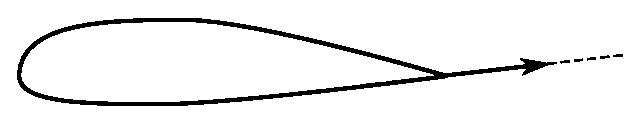
\includegraphics[width=0.3\textwidth]{bottomkutta}
  \caption{Alternative orientations of the wake vortex sheet as it separates
  from the trailing edge of the aerofoil.}
  \label{fig:bottomkutta}
\end{figure}

\section{Quoting Something}

The final paragraph in this chapter illustrates a quote. To do a quote
simply use the enviroment
\begin{verbatim}
\begin{quote}
 The quote text.
\end{quote}.
\end{verbatim}
Note that the edengths class forces quotes to single spacing as the thesis
regulations demand this. Also, there is an inline citation in the next
paragraph.

Lorem ipsum dolor sit amet, consectetur adipiscing elit. Pellentesque id mi sit
amet mauris elementum sagittis eget at neque. Quisque id sapien magna, et
pharetra enim. Aenean congue turpis et libero faucibus vitae vulputate erat
facilisis. Pellentesque \citet[2008]{CCC:2008} iaculis orci a nisl scelerisque
quis accumsan sem viverra. In nec risus dolor, vitae adipiscing erat. Etiam
ultrices leo eget arcu faucibus congue. Nullam eget iaculis mauris. Ut gravida
rutrum nisl eget auctor. Donec sodales enim at massa porta nec mattis est
dapibus. Nunc nec vehicula tellus. Quisque massa tellus, lobortis vel sodales
sed, aliquet varius dui. Proin tincidunt sollicitudin sagittis. 
\begin{quote}
 ``Lorem ipsum dolor sit amet, consectetur adipiscing elit. Pellentesque id mi
sit amet mauris elementum sagittis eget at neque. Quisque id sapien magna, et
pharetra enim. Aenean congue turpis et libero faucibus vitae vulputate erat
facilisis.''
\end{quote}
Lorem ipsum dolor sit amet, consectetur adipiscing elit. Pellentesque id mi sit
amet mauris elementum sagittis eget at neque. Quisque id sapien magna, et
pharetra enim. Aenean congue turpis et libero faucibus vitae vulputate erat
facilisis. Pellentesque iaculis orci a nisl scelerisque quis accumsan sem
viverra. In nec risus dolor, vitae adipiscing erat. Etiam ultrices leo eget arcu
faucibus congue. Nullam eget iaculis mauris. Ut gravida rutrum nisl eget auctor.
Donec sodales enim at massa porta nec mattis est dapibus. Nunc nec vehicula
tellus. Quisque massa tellus, lobortis vel sodales sed, aliquet varius dui.
Proin tincidunt sollicitudin sagittis. 


% \part{The Two Flowers}

\chapter{Another Chapter}

\section{The first section}

Note that all section and chapter titles should use lower case except
for the first character of the first word. Here is a reference to a
paper~\cite{apaper}. Figure~\ref{fig:picture} is a weird picture.

\begin{figure}[h]
  \centering
  %% Because graphicspath was set in edengths.tex you only need to
  %% supply the file name here, i.e. examplepicture (doesn't need the
  %% extension) and not the full path. Just remember to add the path
  %% to \graphicspath{{thispath/}{thatpath/}}
  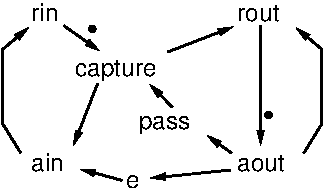
\includegraphics[width=2in]{examplepicture}
  \caption[Long caption and \textit{some italics} to see what happens]%
  {This is an example of pdf with a very long caption and \textit{some italics}
  to see what happens and it should see what happens over two lines.}
\label{fig:picture}
\end{figure}

\subsection{A subsection}

Lorem ipsum dolor sit amet, consectetur adipiscing elit. Maecenas nec orci 
lacus, ac sollicitudin tortor. Maecenas rutrum vestibulum rhoncus. Vestibulum 
non ligula nibh. Cum sociis natoque penatibus et magnis dis parturient montes, 
nascetur ridiculus mus. Phasellus egestas sodales lacus, ac scelerisque nulla 
venenatis sed. Ut elementum turpis ac lacus consectetur consequat. Sed at est 
eros. Praesent erat velit, dictum id adipiscing eu, ultrices vel nisi. Nullam 
at nisl ut est posuere commodo tincidunt eget nisl. Integer id erat non metus 
adipiscing dignissim quis sed enim. Curabitur viverra lobortis eleifend. Proin 
vestibulum nunc eu augue dapibus quis porttitor ipsum rhoncus. Duis tortor 
tellus, suscipit sit amet ornare id, lacinia sed lacus. Ut in molestie ligula. 
Praesent euismod lectus vitae arcu malesuada tempus. Aliquam pharetra 
tincidunt augue in eleifend. Curabitur porttitor vulputate quam, ut fringilla 
mauris porta eu. Curabitur sodales, felis non vestibulum feugiat, urna diam 
bibendum purus, ac scelerisque massa eros sit amet ipsum. In elementum laoreet 
aliquam.

\subsubsection{A subsubsection}

Aliquam eget sapien tellus, sed rutrum leo. Vestibulum et quam sit amet dolor 
gravida sagittis. Aenean dapibus urna a nibh sollicitudin pharetra. Sed nisi 
augue, vehicula sed tristique facilisis, lacinia ut augue. Nam quis tempor mi. 
Vestibulum lorem leo, aliquet at sollicitudin vitae, fringilla id odio. Aenean 
a orci odio. Mauris tincidunt eros ac libero suscipit molestie. Donec feugiat 
turpis a urna suscipit in pellentesque magna pretium. Vivamus eget nunc vitae 
nunc ultricies tincidunt. Duis dictum eros et lorem auctor id ullamcorper diam 
commodo. Pellentesque quis dolor nec urna vestibulum pellentesque. Donec 
luctus mi ut nisi hendrerit pulvinar. Donec fringilla, lectus vitae accumsan 
sollicitudin, sem metus mollis risus, nec laoreet ante arcu ut augue.

\subsection{Another subsection}

Table~\ref{tab:atable} is an example of a~\footnote{this is a
footnote} simple table.

\begin{table}[htb]
\begin{center}
\begin{tabular}{|c|c|c|}
\hline
1.0 & 2.0 & 3.0 \\
\hline
4.0 & 5.0 & 6.0 \\
\hline
\end{tabular}
\caption{A table}
\label{tab:atable}
\end{center}
\end{table}


\section{Another section}

This is a long and boring paragraph for the purpose of testing the
spacing between paragraphs and the use or otherwise of indentation. I
think a space between paragraphs and without the first line indented
is somewhat easier to read than no space between paragraphs and with
the first line indented.

Another equally exciting paragraph, one two three four five six seven
eight nine ten eleven twelve thirteen fourteen fifteen sixteen
seventeen eighteen nineteen twenty and so on.

\begin{equation} \label{eqn:dct}
z(k,l) = \frac{2}{N} \alpha(k) \alpha(l) \sum_{m=0}^{N-1} \sum_{n=0}^{N-1}
         x(m,n) \cos \frac{ (2m+1) \pi k}{2N} \cos \frac{ (2n+1) \pi l}{2N}
\end{equation}

\begin{equation} \label{eqn:idct}
x(m,n) = \frac{2}{N} \sum_{k=0}^{N-1} \sum_{l=0}^{N-1}
         \alpha(k) \alpha(l) z(k,l)
\end{equation}

\begin{quotation}
This is a quotation, another equally exciting paragraph, one two three
four five six seven eight nine ten eleven twelve thirteen fourteen
fifteen sixteen seventeen eighteen nineteen twenty and so on. Just
checking it is single spaced.
\end{quotation}

\section{Section with a landscape image}

\Autoref{fig:landscape} is an image on a landscape orientated page with
the header removed and a simple footer added.

\begin{landscape}
\thispagestyle{plain} % Remove this line for normal headers
\begin{figure}[p]
  \centering
    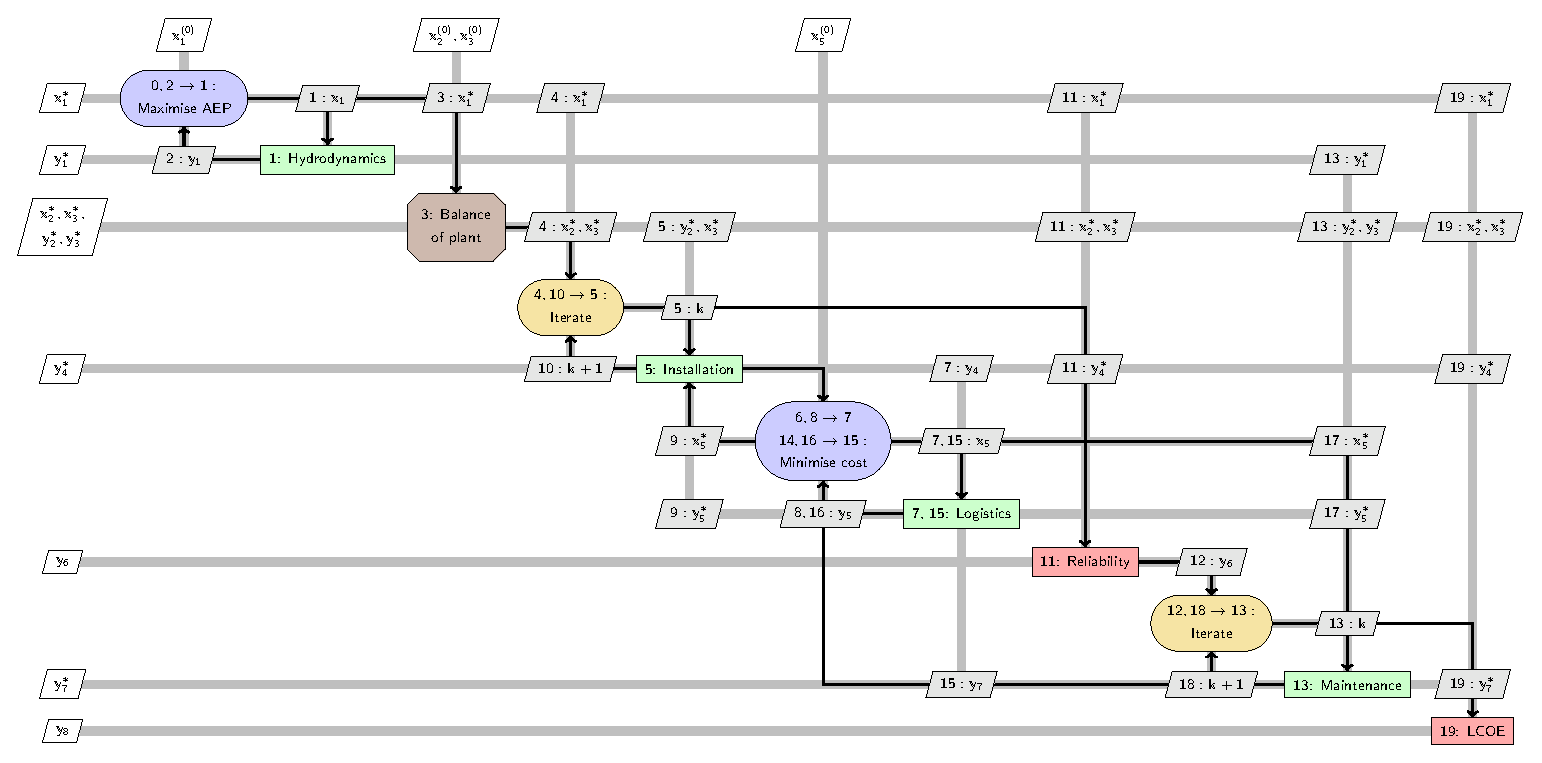
\includegraphics[width=\linewidth]{xdsm_sequential-crop}
    \caption{XDSM diagram. Reproduced from \citep{topper2021}.
    \label{fig:landscape}
}
\end{figure}
\end{landscape}

% \include{chapter3/chapter3}
% \include{chapter4/chapter4}
% \include{chapter5/chapter5}
% \include{chapter6/chapter6}

%%%% START APPENDICIES

%% Execute the appendix commands. To allow use of include
%% for appendix files, the commands are maintained in a
%% separate file.
%%
%% This file must also be listed in the \includeonly command.
%%
%% edengapp.tex - Addition to edength Latex2e thesis class
%%
%% Copyright (C) 2010-2017 Mathew Topper <damm_horse@yahoo.co.uk>
%%
%%
%%   ABOUT
%%
%% This is required to start the appendicies for a Latex2e template which
%% corresponds to the regulations regarding layout of a thesis submitted
%% within the University of Edinburgh.

%%%% START APPENDIX

%% These commands must be '\included' to '\include' the appendx.tex files.
\appendix

%% Add appendicies heading to the TOC but without a number
\noappendicestocpagenum
\addappheadtotoc

%% Change 'Chapter' to 'Appendix'
\renewcommand{\chaptername}{Appendix}

%% Equations should have the chapter letter in them.
\renewcommand{\theequation}{\Alph{chapter}.\arabic{equation}}


%% Appendix files. Start each with \chapter
\chapter{Insert appendix title here}
\label{append:model}

\section{Mathematical explanation of the effect of restricting the enzyme pool}
\label{append:model-pool}

Let $\ratioabl$, given by equation~\ref{eq:model-ratio}, depend on $x$:

\begin{equation}
  \ratioabl(x) = \left( \sum_i \frac{f_i}{\griabl(x)} \right) \cdot \frac{\gro(x)}{\biomfrac{protein}}
  \label{eq:model-ratio-x}
\end{equation}

where $x = \epool^{\prime}/\epool$.
The expression in Eq.\ \ref{eq:model-ratio-x} takes into account how $\gro$ and $\griabl$ values vary with $x$, and how $f_{i}$ values are constants.

We thus obtain:
\begin{equation}
  \begin{aligned}
  \ndif{\ratioabl(x)}{x} &= \frac{1}{\biomfrac{protein}} \ndif{}{x} \left[ \left( \sum_i \frac{f_i}{\griabl(x)} \right) \cdot \gro(x) \right]\\
  &= \frac{1}{\biomfrac{protein}} \left[ \left( \sum_i \frac{f_i}{\griabl(x)} \right) \cdot \ndif{\gro(x)}{x} + \gro(x) \ndif{}{x} \left( \sum_i \frac{f_i}{\griabl(x)} \right) \right]\\
  &= \frac{1}{\biomfrac{protein}} \left[ \left( \sum_i \frac{f_i}{\griabl(x)} \right) \cdot \ndif{\gro(x)}{x} - \gro(x) \sum_{i}\left( \frac{f_{i}}{\griabl(x)^{2}} \cdot \ndif{\griabl(x)}{x} \right) \right]
  \end{aligned}
  \label{eq:model-ratio-diff}
\end{equation}

To explain the increase in $\ratioabl$ as $\epool^{\prime}$ increases, I consider the behaviour of $\gro$ and $\griabl$ values with respect to $\epool^{\prime}$ in intervals.

With reference to Fig.\ \ref{fig:model-pool}, consider $0 \leq x \leq 0.5$.
In this region of $x$, based on the observations in the figure, we model $\gro = k_{0}x$ and $\griabl = k_{i}x$, where constants $k_{0}, k_{i} > 0$.
This models how these values initially increase linearly in figure~\ref{fig:model-pool}.
Equation~\ref{eq:model-ratio-diff} thus becomes:
\begin{equation}
  \begin{aligned}
  \ndif{\ratioabl(x)}{x} &= \frac{1}{\biomfrac{protein}} \left[ \left( \sum_i \frac{f_i}{k_{i}x} \right) \cdot k_{0} - k_{0}x \sum_{i}\left( \frac{f_{i}}{(k_{i}x)^{2}} \cdot k_{i} \right) \right]\\
  &= \frac{1}{\biomfrac{protein}} \left[ \frac{k_{0}}{x} \sum_i \frac{f_i}{k_{i}} - k_{0}x \left( \sum_{i} \frac{f_{i}}{k_{i}x^{2}} \right) \right]\\
  &= \frac{1}{\biomfrac{protein}} \left[ \frac{k_{0}}{x} \sum_i \frac{f_i}{k_{i}} - \frac{k_{0}}{x} \sum_i \frac{f_i}{k_{i}} \right]\\
  &= 0
  \end{aligned}
  \label{eq:model-ratio-diff-smallx}
\end{equation}

And this explains the constant $\ratioabl$ in this region.

Now, consider $0.5 < x \leq 9$.
In this region, the trajectories of $\griabl$ with respect to time remain linear, but some with changes in slope.
In other words, in a sub-region where the slopes of all $\griabl$ are constant, we can let: $\gro = k_{0}x$ and $\griabl = m_{i}x + c_{i}$, where $k_{0}, m_{i}, c_{i} > 0$.
Equation~\ref{eq:model-ratio-diff} thus becomes:
\begin{equation}
  \begin{aligned}
  \ndif{\ratioabl(x)}{x} &= \frac{1}{\biomfrac{protein}} \left[ \left( \sum_i \frac{f_i}{m_{i}x+c_{i}} \right) \cdot k_{0} - k_{0}x \sum_{i}\left( \frac{f_{i}}{(m_{i}x+c_{i})^{2}} \cdot m_{i} \right) \right]\\
  &= \frac{k_{0}}{\biomfrac{protein}} \left[ \left( \sum_i \frac{f_i}{m_{i}x+c_{i}} \right) - x \left( \sum_{i} \frac{f_{i}m_{i}}{(m_{i}x+c_{i})^{2}} \right) \right]\\
  &= \frac{k_{0}}{\biomfrac{protein}} \sum_{i} \left[ \frac{f_i}{m_{i}x+c_{i}} - \frac{xf_{i}m_{i}}{(m_{i}x+c_{i})^{2}} \right]\\
  &= \frac{k_{0}}{\biomfrac{protein}} \sum_{i} \left[ \frac{f_{i}c_{i}}{(m_{i}x+c_{i})^{2}} \right]
  \end{aligned}
  \label{eq:model-ratio-diff-midx}
\end{equation}

As $f_{i}, c_{i}, m_{i} > 0$ for all biomass components $i$, and $k_{0} > 0$, we get $\ndif{\ratioabl(x)}{x} > 0$ regardless of the values that these constants take.
Because $k_{0}$ does not change over the region of $x$ considered, $m_{i}$, $c_{i}$, and $x$ values thus determine the magnitude of $\ndif{\ratioabl(x)}{x}$.
If within a region of $x$, $m_{i}$ and $c_{i}$ values remain constant for all $i$, then as $x$ increases, $\ndif{\ratioabl(x)}{x}$ should decrease --- this is certainly the case, as can be observed in figure~\ref{fig:model-pool}.

Lastly, consider $x > 9$.
In this region, $\gro$ becomes constant, thus we let $\gro = k_{0}$.
We keep $\griabl = m_{i}x + c_{i}$, and as before, $k_{0}, m_{i}, c_{i} > 0$.
Equation~\ref{eq:model-ratio-diff} thus becomes:
\begin{equation}
  \begin{aligned}
  \ndif{\ratioabl(x)}{x} &= \frac{1}{\biomfrac{protein}} \left[ 0 - k_{0} \sum_{i}\left( \frac{f_{i}}{(m_{i}x+c_{i})^{2}} \cdot m_{i} \right) \right]\\
  &= -\frac{k_{0}}{\biomfrac{protein}} \sum_{i}\left[ \frac{f_{i}m_{i}}{(m_{i}x+c_{i})^{2}} \right]
  \end{aligned}
  \label{eq:model-ratio-diff-largex}
\end{equation}

This predicts \emph{decreasing} $\ratioabl$ as $x$ increases in this region.
Because $k_{0}$ is constant in this region, the rate of this decrease is thus controlled by $m_{i}$ and $c_{i}$ values.
As each $\griabl$ trajectory becomes flat as $x$ increases, each $\frac{f_{i}m_{i}}{(m_{i}x+c_{i})^{2}}$ term becomes zero, thus shrinking the magnitude of $\ndif{\ratioabl(x)}{x}$.
Finally, as all $\griabl$ trajectories become flat at $x > 15$, $\ndif{\ratioabl(x)}{x} = 0$.

% \include{appendix/appendx2}


%%%% WRITE OUT BIBLIOGRAPHY

%% Path to bib file. Use \edbibliography command here or the
\edbibliography{bib/edengref}

%% Path to style file. It's recommended that you use the provided style
%% file (a variation on plainnat) as it does italic et als and reduces
%% all first names to initials. It also puts the surname first in apa style.
\bibliographystyle{apacite}

\end{document}
